A de Bruijn sequence, or a positioning sequence, (of order $k$) is a binary sequence in which every possible length-$k$ string appears exactly once as a substring. The uses of de Bruijn sequence has been found in various field. Recently, a novel application of positioning sequences has been found in quantum communication by \citeauthor{zhang2021timing}. They adapt such sequences into \gls{HdB} sequences to develop a system for synchronising in quantum channels. Though having shown advantages against other methods~\cite{zhang2021timing}, such implementation still has drawbacks and there are rooms for improvements. This thesis focuses on designing a new constrained de Bruijn sequence and proving its efficiency against \gls{HdB} sequence. 

Chapter \ref{chapter:motivation} first briefly introduces the \gls{qkd} protocol, along with the reasonable motivation to study the synchronization mechanisms in satellite quantum channels. Among such mechanisms, the timing and synchronization system proposed by \citeauthor{zhang2021timing} in~\cite{zhang2021timing} is analyzed to recognise its disadvantages. After that, the main results of this thesis, which aim to improve those weaknesses, is summarized. The organization of the whole thesis is given in the end of this chapter. 

% Chapter \ref{chapter:motivation} introduces a de Bruijn based system used in Quantum communication. The drawback of this system is the inspiration for the results in this thesis. This thesis's contributions are also summarized in this chapter. 

\section{Timing and synchronization de Bruijn based system}
Symmetric, public-key (asymmetric), and hash-based cryptography are fundamental pillars of modern cryptography. While  symmetric schemes and hash functions are less vulnerable to quantum attacks, the asymmetric schemes based on factoring or solving the discrete logarithm problem, for example: Rivest-Shamir-Adelman (RSA), Elliptic Curve Cryptography, are completely broken by a quantum adversary via Shor's algorithm~\cite{shor1999polynomial}. Currently deployed public key cryptosystems are used to establish a common secret key between two parties. Doing the same jobs, \gls{qkd} enables two parties to produce a shared random secret key known only to them. Moreover, \gls{qkd} is able to guarantee the security of communication links making them immune to quantum computer-based attacks~\cite{gheorghiu2019benchmarking}. 

The first invented \gls{qkd} protocols are BB84~\cite{bennett1984quantum}, and E91~\cite{ekert1992quantum}. Since 2005, \gls{qkd} has been initially implemented in real life. For example, in 2005, University of Geneva and Corning Inc used a fiber optic wire of $307$ km. In 2007, Los Alamos National Laboratory and the National Institute of Standards and Technology (NIST) used the BB84 protocol over a 148.7 km optical fiber. In 2018, Quantum Xchange launched the first quantum network in the U.S., offering $1,000$ km of fiber optic cable and 19 colocation centers along the Boston-to-Washington, D.C., corridor and metro hubs. However, due to the intrinsic exponential losses over optical fiber, the deployed \gls{qkd} systems' range is restricted to under $1000$ km. So as to establish intercontinental secure communication links, which usually requires a range over $1000$ km, satellite \gls{qkd} has been proposed as an alternative, with the pioneering Micius satellite. In these systems, the transmitter (satellite) and the receiver (optical ground station) relentless exchange information after measuring the quantum states. But transmitting faint quantum optical pulses between a satellite and the Earth is challenging due to high channel losses cause by volatility environment and rapid relative motion between two parties. 

To deal with this problem, the reliable and efficient timing and synchronization systems have been proposed in~\cite{khader2018time,duan2021survey}. In this system, a classical channel is used along with the quantum channel, because of its advantage in synchronization. Figure~\ref{fig:qkd_satellite} shows a high-level view of this schematic.

\begin{figure}[htbp]
    \centering
    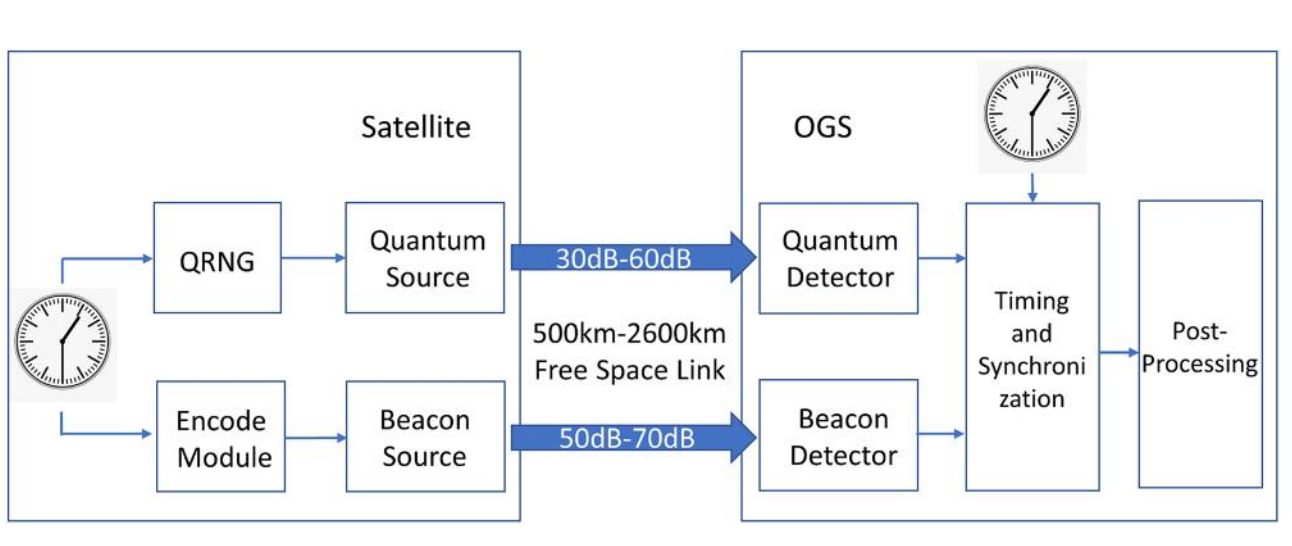
\includegraphics[scale=0.3]{fig/SatelliterQKD.png}
    \caption{High-level satellite Quantum Key Distribution timing and synchronization schematic \cite{zhang2021timing}.}
    \label{fig:qkd_satellite}
\end{figure}

Based on that concept, in~\cite{zhang2021timing}, a \gls{dBTS} is introduced using a beacon with on-off model. In this model, a de Bruijn sequence is transmitted from the satellite to the ground for synchronization. 

The encode process happens at the satellite, where it uses the \gls{lfsr} algorithm to generate a positioning sequence (of order $k$ for example). The prerequisite of finding a proper primitive polynomial is the main drawback of this encoder. 

The decode process takes place at the ground station, a look-up table is used to identify the unique position of the received sequences of length $k$. The complexity of this method is exponential.

Furthermore, in this model, a sequence of beacon pulses are used to represent a binary de Bruijn sequence. Considering the timing jitter performance, a long period of no-pulses should be forbidden. If one pulse slot is used to represent a binary bit, for example, on is 1 and off is 0, a long run of 0's in the sequence (which is a long period of no-pulses) would impact the timing jitter. In \cite{zhang2021timing}, two pulse slots are used to represent a single bit, on-on is 1 and on-off is 0, so that one can avoid two consecutive no-pulses. The transmitted sequence is called \gls{HdB}. However, the above scheme requires $2n$ pulse slots to represent a de Bruijn sequence of length $n$ and needs to receive a sub-sequence of $2 \log n$ pulse slots to locate its position. Formally, the \gls{HdB} sequence's rate is just $0.5$, where rate is a quantity that needs to be as high as possible (the definition of sequences' rate is given in section \ref{sec:rate}).

% For further illustration, the whole process, methods, and drawbacks of \gls{dBTS} system using \gls{HdB} sequence is summarized is figure \ref{fig:dBTS}
% \begin{figure}[htbp]
%     \centering
%     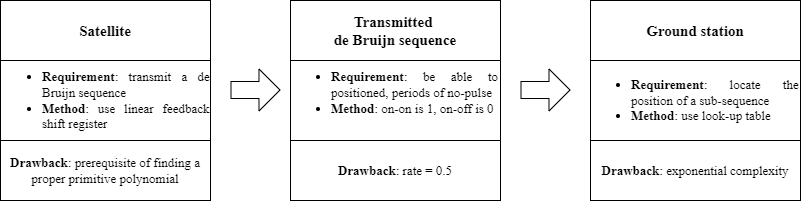
\includegraphics[scale=0.5]{fig/dBTS.png}
%     \caption{de Bruijn based timing and synchronizing system use Hybrid de Bruijn code}
%     \label{fig:dBTS}
% \end{figure}

Table \ref{tab:dBTS} summarized the process, applied methods and drawbacks of \gls{dBTS} system using \gls{HdB} sequence.
\begin{table}[htbp]
    \centering
    \caption{Timing and synchronizing system use Hybrid de Bruijn code.}
    \renewcommand{\arraystretch}{1.25}
    \resizebox{\columnwidth}{!}{
    \begin{tabular}{| p{4.1cm} | p{4.1cm}| p{4.1cm} |}
    % \begin{tabular}{|l|l|l|}
        \hline
        \textbf{Satellite} & \textbf{Transmited de Bruijn sequence} & \textbf{Ground Station} \\
        \hline \hline
        \textbf{Requirement}: transmit a de Bruijn sequence of order $k$
          &
        \textbf{Requirement}: be able to be positioned, avoid periods of no-pulse 
          &
        \textbf{Requirement}: locate the position of any length $k$ subsequence  \\
        \hline
        \textbf{Method}: use linear feedback shift register algorithm
          &
        \textbf{Method}: modulate on-on is $1$, on-off is $0$
          &
        \textbf{Method}: use look-up table \\
         \hline 
        \textbf{Drawback}: the prerequisite of finding a proper primitive polynomial 
        &
        \textbf{Drawback}: rate is $0.5$
        &
        \textbf{Drawback}: exponential complexity \\
        \hline
    \end{tabular}
    }
    \label{tab:dBTS}
    
\end{table}

% \begin{table}[htbp]
%     \centering
%     \begin{tabularx}{\textwidth} { 
%   | >{\raggedright\arraybackslash}X 
%   | >{\raggedright\arraybackslash}X 
%   | >{\raggedright\arraybackslash}X | }
%  \hline
%         \textbf{Satellite} & \textbf{Transmited de Bruijn sequence} & \textbf{Ground Station} \\
%          \hline 
%         \textbf{Requirement}: transmit a de Bruijn sequence of order $k$
%           &
%         \textbf{Requirement}: be able to be positioned, avoid periods of no-pulse 
%           &
%         \textbf{Requirement}: locate the position of any length $k$ subsequence  \\
%         \hline 
%         \textbf{Method}: use linear feedback shift register algorithm
%           &
%         \textbf{Method}: modulate on-on is $1$, on-off is $0$
%           &
%         \textbf{Method}: use look-up table \\
%          \hline 
%         \textbf{Drawback}: the prerequisite of finding a proper primitive polynomial 
%         &
%         \textbf{Drawback}: rate is $0.5$
%         &
%         \textbf{Drawback}: exponential complexity \\
%         \hline
% \end{tabularx}
%     \caption{Caption}
%     \label{tab:my_label}
% \end{table}





\section{The contributions and organization of this thesis}
This thesis aims to improve the drawback of the \gls{HdB} sequence listed above. The main task here is designing a code satisfying the constraints of \gls{dBTS} system.

\textbf{Problem Statement}: Designing a high rate sequence which is capable of positioning and avoids two consecutive symbol $0$'s.

Chapter \ref{chapter:RdB} presents the proposed sequence of this thesis, which is called Run length limited de Bruijn sequence (\gls{RdB}). The \gls{RdB} sequence is not just suitable with \gls{dBTS} system, but also have a higher rate than \gls{HdB} sequence. More precisely, rate of the longest \gls{RdB} sequence is \[\log\left(\dfrac{1+\sqrt{5}}{2}\right)\approx0.6942.\]

Chapter \ref{chapter:pro_rlldb_sequence} provides the efficient algorithm to generate one of the longest \gls{RdB} sequence. This algorithm, called an encoder, is based on the \gls{fkm}, which is the fastest method to produce a de Bruijn sequence. Moreover, to locate the position of an abitrary proper subsequence in the whole \gls{RdB} sequence, a decoder is also presented. The proposed decoder modifies the decoding algorithm found by Kociukima .et.al in \cite{kociumaka2016efficient}, which is currently the state of the art method to position a subsequence in the de Bruijn sequence, and therefore, is better than look-up table.

Beside, the \gls{RdB} sequence is even more general and adaptive. More particularly, when the constraint of forbidding pattern $00$ is relaxed, that is, a longer run of bit $0$'s is allowed, the \gls{RdB} sequence can be easily adjusted to make the its rate higher and still suits the system. 

In summary, the contributions of this thesis is listed as follows:
\begin{itemize}
    \item Proposing a new kind of sequence (\gls{RdB}), more efficient (higher rate, more general and adaptive) than \gls{HdB} sequences.
    \item Determining the length of the longest \gls{RdB} sequence.
    \item Providing fast encoder and decoder based on state of the art algorithms.
\end{itemize}

% Chương này có độ dài không quá 10 trang. Chương này sinh viên trình bày về phân tích rõ ngữ cảnh bài toán cũng như các kết quả nghiên cứu tương tự. Đồng thời, sinh viên có thể trình bày thêm về các kiến thức nền tảng.

% \section{Scope of Research}
% \ldots

% \section{Related Works}
% Trong phần này sinh viên trình bày các nghiên cứu liên quan (related work), chú ý phân tích rõ những ưu nhược điểm của chúng. Từ đó, nêu bật lên động lực để thực hiện nghiên cứu của đồ án này.


% \section{Tên của kiến thức nền tảng số 1}
% Tiêu đề và nội dung của chương này sẽ thay đổi tuỳ thuộc vào từng đồ án. Chú ý trình bày những kiến thức có liên quan mật thiết nhất đối với đồ án của mình, Tránh trình bày lan man những kiến thức phổ thông không cần thiết. 

% \section{Tên của kiến thức nền tảng số 2}
% Tiêu đề và nội dung của chương này sẽ thay đổi tuỳ thuộc vào từng đồ án. Chú ý trình bày những kiến thức có liên quan mật thiết nhất đối với đồ án của mình, Tránh trình bày lan man những kiến thức phổ thông không cần thiết. 